\ifdefined\standalone 
\documentclass[12pt]{article}
\usepackage{graphicx}
\usepackage{float}
\usepackage[a4paper, margin=1in]{geometry}
\usepackage[utf8]{inputenc}
\usepackage{textcomp}
\usepackage{amsmath}
\usepackage{booktabs}
\usepackage{tikz}
\usepackage{enumitem}
\usetikzlibrary{decorations.pathmorphing,patterns}
\usepackage[hidelinks]{hyperref} % <- hypertext
\usepackage{caption}

\begin{document}
\fi

\section{In-Depth Radiation With Surface Convection}

This verification case assesses the ability of Gpyro to represent one-dimensional heat absorption due to volumetric radiation combined with surface cooling by convection. A slab of thickness $L = 10~\mathrm{cm}$ is considered.The thermophysical properties of the material are summarized in Table~\ref{tab:rad_conv_phys_props}. The top surface is subjected to convective heat transfer with a constant convective heat transfer coefficient of $h_c = 10~\mathrm{W\,m^{-2}\,K^{-1}}$ and an ambient gas temperature of $T_\infty = 25~^\circ\mathrm{C}$. In addition, the top surface is also exposed to an external radiative heat flux of $q''_\mathrm{ext} = 5~\mathrm{kW\,m^{-2}}$.The material is assumed to be semi-transparent, characterized by an absorption coefficient of $\kappa = 24~\mathrm{m^{-1}}$. The bottom surface of the slab is assumed to be adiabatic. The initial temperature is uniform throughout the material, with $T_{ini} = 25~^\circ\mathrm{C}$. The configuration is illustrated in Fig.~\ref{fig:rad_conv_temp}.

An analytical solution for transient temperature evolution within the slab is available and is taken from the formulation presented in Lautenberger’s thesis \cite{lautenberger2007}:

\begin{equation}
\label{eq:temp_depth_lautenberger}
\begin{aligned}
T(z) - T_{ini} &= \frac{2 \varepsilon q''_\mathrm{ext} \kappa^2}{k}
\sum_{m=1}^{\infty} \frac{1}{\lambda_m (\kappa^2 + \lambda_m^2)} \\
&\quad \times
\frac{\cos(\lambda_m L) + \tfrac{\lambda_m}{\kappa} \sin(\lambda_m L) - \exp(-\kappa L)}
{\lambda_m L + \tfrac{1}{2} \sin(2 \lambda_m L)} \\
&\quad \times
\cos\!\bigl(\lambda_m (L - z)\bigr)
\left(1 - \exp(-\alpha \lambda_m^2 t)\right)
\end{aligned}
\end{equation}

The eigenvalues $\lambda_m$ are obtained by solving the following equation:

\begin{equation}
\label{eq:lambda_condition}
\cot(\lambda_m L) = \frac{k}{h_c}\,\lambda_m
\end{equation}


\begin{table}[H]
\centering
\caption{Material properties}
\label{tab:rad_conv_phys_props}
\renewcommand{\arraystretch}{1.2}
\begin{tabular}{c c c c c}
\hline
$k$ ($\mathrm{W\,m^{-1}\,K^{-1}}$) &
$c_p$ ($\mathrm{J\,kg^{-1}\,K^{-1}}$) &
$\rho$ ($\mathrm{kg\,m^{-3}}$) &
$\varepsilon$ &
$\kappa$ (m$^{-1}$) \\
\hline
0.10 & 1000 & 100 & 1 & 24 \\
\hline
\end{tabular}
\end{table}


\begin{figure}[H]
\centering

\begin{minipage}[t]{0.45\textwidth}
\centering
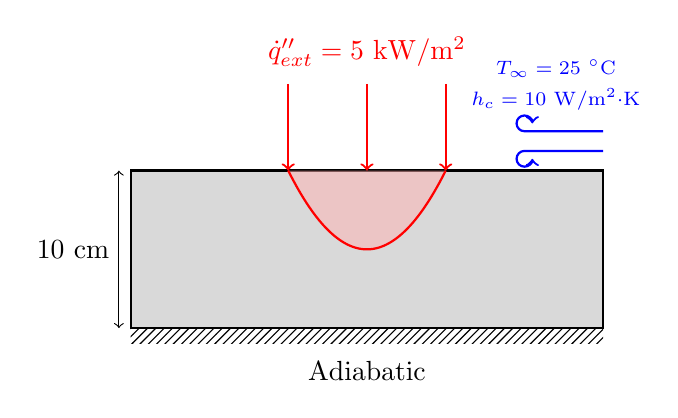
\begin{tikzpicture}[scale=1.0]
% MDF block
\draw[fill=gray!30,thick] (0,0) rectangle (6,2); 

% Adiabatic bottom
\fill[pattern=north east lines] (0,-0.2) rectangle (6,0);
\node[below] at (3,-0.3) {Adiabatic};

% Dimension line for height
\draw[<->] (-0.15,0) -- (-0.15,2);
\node[left] at (-0.15,1) {10~cm};

\foreach \x in {1.8,2.8,3.8}
    \draw[->,thick,red] (\x+0.2,3.1) -- (\x+0.2,2);

\node[above,red] at (3,3.2) {$\dot{q}''_{ext} = 5~\mathrm{kW/m^2}$};

\draw[->,thick, blue] (6,2.25) -- (5,2.25) arc[start angle=90, end angle=360, radius=0.1cm]; 
\draw[->,thick, blue] (6,2.5) -- (5,2.5) arc[start angle=270, end angle=0, radius=0.1cm];

\node[blue] at (5.4,2.9) {\scriptsize $h_c = 10~\mathrm{W/m^2{\cdot}K}$};
\node[blue] at (5.4,3.3) {\scriptsize $T_\infty = 25~^\circ\mathrm{C}$};

\fill[red!30, opacity=0.5, domain=2:4, variable=\x] (2,2) plot ({\x}, {(\x-3)^2 + 1}) --(4,2) -- cycle;

\draw[thick, red, domain=2:4, samples=100, smooth, variable=\x] plot ({\x}, {(\x-3)^2 + 1});

\end{tikzpicture}
\caption{Configuration schematic}
\label{fig:rad_conv_configuration}
\end{minipage}
\hfill
\begin{minipage}[t]{0.45\textwidth}
\centering
    \includegraphics[width=\linewidth]{temperature_results.png}
    \caption{Temperature evolution at different points in the slab}
\label{fig:rad_conv_temp}
\end{minipage}
\end{figure}

\ifdefined\standalone
\end{document}
\fi






